\documentclass{../template/mai_book}

\defaultfontfeatures{Mapping=tex-text}
\setmainfont{DejaVuSerif}
\setdefaultlanguage{russian}

\clearpage
\setcounter{page}{444}
\setcounter{thm}{19}
\setcounter{section}{3} % ТАК ЗАДАВАТЬ ГЛАВЫ, ПАРАГРАФЫ И ПРОЧЕЕ.
% Эти счетчики достаточно задать один раз, обновляются дальше сами
\setcounter{subsection}{2}



\usepackage{amsmath}
\begin{document}
%\lhead{444}
%\rhead{IV-3 \small\textit{Группа обратимых элементов}}
\noindent обратно к $3$ по модулю $(p — 1)(q — 1)$. Возводя полученное сообщение в\linebreak
степень $d$ по модулю $n$, получатель найдет число $m$.

Чтобы завершить обсуждение RSA, отметим, что до настоящего\linebreak
времени все сколько-нибудь серьезные атаки на RSA были либо не­-\linebreak
корректными, либо сводились к алгоритму факторизации целых чисел.\linebreak
Эквивалентность между этими двумя проблемами, кстати, в общем слу­-\linebreak
чае не доказана (см. Рабин [151]).

Хотя систему RSA очень трудно атаковать, но зато можно получить\linebreak
некоторую частичную информацию. В частности, некоторые свойства\linebreak
шифруемых элементов могут быть снова найдены в криптограммах.\linebreak
Например, свойство числа из $\mathbb{Z}/n\mathbb{Z}$ быть квадратичным вычетом со-\linebreak
храняется при зашифровке.

\paragraph{3.2.2 Алгоритм рюкзака}
\subparagraph{}Этот метод опирается на алгоритмическую сложность хорошо из-\linebreak 
вестной проблемы и принадлежит Мерклю и Хеллману [127]. Свое на­-\linebreak
звание метод получил благодаря во многом аналогичной проблеме, ко-\linebreak
торая возникает у путешественника, имеющего рюкзак и желающего\linebreak
унести как можно больше вещей из $n$ имеющихся, которые, к сожале-\linebreak
­нию, все в рюкзак не умещаются. Следовательно, он должен выбрать\linebreak
предметы, чтобы наиболее оптимально наполнить рюкзак. Более фор-\linebreak
­мально, общая проблема состоит в следующем: дана $n$-ка положитель-\linebreak
ных целых чисел $(a_1, a_2,...,a_n)$ и положительное число $S$ такое, что\linebreak
$S=\sum a_i x_i$, c $x_i \in \{0, 1\}$. Если вычисление $S$, при известных $x_i$, очень\linebreak
простая процедура, требующая всего $n$ сложений, то поиск $x_i$, для за-\linebreak
данных $S$ и $a_i$, требует порядка экспоненты от $n$ операций, если числа $a_i$\linebreak
не выбраны особым образом (поставленная задача является $N P$-полной,\linebreak
как и классическая задача коммивояжера).

Следовательно, в общем случае эту проблему решить невозможно, а\linebreak значит, можно адаптировать алгоритм рюкзака для получения функ-\linebreak
­ции ловушки. Для этого, конечно, нужно выделить класс $n$-ок, для\linebreak
которых, имея некоторую дополнительную информацию (секретную),\linebreak
можно решить проблему рюкзака. Во всяком случае, следует отметить,\linebreak
что решение этой проблемы существует не всегда, а если решение су-\linebreak
ществует, то оно не обязательно единственно.
\begin{determ}
$n$-ка положительных чисел $(b_1,b_2,...,b_n)$ называется сверхрастущей,\linebreak если каждая компонента $b_i$ больше суммы всех предыдущих.
\end{determ}
Проблема рюкзака легко решается для сверхрастущей $n$-ки чисел.\linebreak
Действительно, пусть $S = \sum x_i b_i$ с $x_i = 0$ или $1$. Начнем с поиска\linebreak
\noindent в $n$-ке $b$ наибольшего элемента, меньшего $S$, скажем $b_k$. Так как $n$-\linebreak
ка $b$ сверхрастущая, то число $S\text{ -- }b_k$ строго меньше, чем $b_k$ и к нему\linebreak
снова можно применить только что описанный процесс. Таким образом,\linebreak
за линейное время можно найти единственное решение проблемы или\linebreak
доказать, что его нет.

Конечно, в этом частном виде, алгоритм рюкзака не представляет\linebreak
никакого интереса для криптографии. Но идея Меркля и Хеллмана со­-\linebreak
стоит в том, чтобы немного изменить компоненты сверхрастущей $n$-ки\linebreak
и получить $n$-ку, по виду не отличающуюся от других, но несущую в\linebreak
себе скрытое сверхвозрастание исходной $n$-ки. Для этого выбирается\linebreak
произвольное число $m$, большее $\sum b_i$ и число $w$, взаимно простое с $m$,\linebreak
обратное к которому по модулю $m$ есть $u$. Далее вычисляем новую $n$-ку\linebreak
$a = (a_1,a_2,...,a_n)$ по правилу $a_i = wb_i (\text{mod} m)$ и в качестве открытого\linebreak
ключа публикуем $а$, а числа $b_i$, $m$ и $w$ держим в секрете. Понятно, что\linebreak
$n$-ка $a$ больше не сверхрастущая (в противном случае $m$ и $w$ выбраны\linebreak
неудачно).

Процесс расшифровки очень прост: лицо, желающее отправить со­-\linebreak
общение, кодирует его при помощи $0$ и $1$, затем разбивает полученную\linebreak
последовательность на группы из $n$ битов, $x_i$, и посылает криптограм-\linebreak­
му $S = \sum x_i a_i$. Дешифровка не менее проста: полученное сообщение\linebreak
$S$ умножаем на $u$ $w$ $S' = \sum x_i b_i$
дальнейшее декодирование тривиально, так как $b$ сверхрастущая.

\noindent\textbf{\textit{Пример}}

Чтобы немного разъяснить механизм действия этой системы, про­
иллюстрируем его на конкретном примере. Возьмем сверхрастущую по­
следовательность $b$ (состоящую из чисел Фибоначчи):

\begin{center}
$5$,\;\;\;\;\;$13$,\;\;\;\;\;$21$,\;\;\;\;\;$89$,\;\;\;\;\;$233$,\;\;\;\;\;$377$,\;\;\;\;\;$987$,\;\;\;\;\;$2 584$,\;\;\;\;\;$6 765$,\;\;\;\;\;$17 711$.
\end{center}

\noindent Сумма этих чисел равна $28 785$ и в качестве модуля $m$, большего этой\linebreak
суммы, выберем наименьшее простое число, большее числа Фибоначчи\linebreak
$46368$, это $m = 46381$. Так как $m$ простое, то любой множитель подхо­-\linebreak
дит для изменения $Ь$, а потому возьмем $w = 522$. Обратное к нему по\linebreak
модулю то есть $u = 40961$. Тогда открытый ключ $а$, полученный из $b$\linebreak
при помощи умножения на $522$, выглядит так:

\begin{center}
$2 610$,\;\;\;\;$6 786$,\;\;\;\;$10 962$,\;\;\;\;$77$,\;\;\;\;$28 864$,

$11 270$,\;\;\;\;$5 023$,\;\;\;\;$3 799$,\;\;\;\;$6 374$,\;\;\;\;$15 323$.
\end{center}
\noindent Теперь рассмотрим три обмена сообщениями между Кларой, которая\linebreak
знает только набор $а$, и Романом, который имеет всю информацию.
\pagebreak
\subparagraph{Сообщение 1}
Допустим Клара хочет послать Роману секретное\linebreak
сообщение $(1,0,1,1,0,1,0,0,0,1)$. Она составляет сумму соответствую­\linebreak
щих элементов из $a$: $S = 40 242$ и посылает ее Роману.\linebreak
Роман умножает полученный криптотекст на $40961$ по модулю\linebreak
$46381$, что дает $S' = 18203$. Далее он ищет в $b$ наибольший элемент,\linebreak
меньший $S'$, — это $b_10 — 17711$, вычитает это число из $S'$ и отмечает,\linebreak
что последний бит сообщения равен 1. Затем Роман ищет наибольшее\linebreak
$b_i$, меньшее $S' = 492$, — это $b_6 = 377$. Таким образом, новые биты со­-\linebreak
общения есть $0$, $0$, $0$ и $1$ ...; продолжая в том же духе, Роман вскоре\linebreak
закончит дешифровку и найдет сообщение, посланное Кларой.

\subparagraph{Сообщение 2}
Роман получает криптограмму $S$ = 91088, умно­-\linebreak
жает ее на 40961 по модулю 46381 и получает $S'$ = 28785. Ага!\linebreak
Это сумма всех элементов из $b$, а значит, было послано сообщение\linebreak$
(1,1,1,1,1,1,1,1,1,1)$.

\subparagraph{Сообщение 3}
Криптограмма — это $S = 40831$. Умножение\linebreak
$S$ на $u$ дает $26112$. Тогда, произведя декодирование, получим $M =\linebreak
(1,1,1,0,1,1,1,0,1,1)$. но это еще не все! Охваченный сомнением, подо­-\linebreak
зрительный по природе Роман, решает зашифровать $М$ , как бы желая\linebreak
послать его самому себе. И к собственному удивлению находит не $S$, а\linebreak
$87 212$. Следовательно, полученная криптограмма не была зашифрована\linebreak
ключом Романа и его пытались обмануть. Конечно, чудес не бывает, и\linebreak
оба сообщения, полученное и найденное Романом, сравнимы по модулю\linebreak
$m$, чем и объясняется возможность дешифровки. Неразбериха происхо­-\linebreak
дит из-за того, что Клара производит вычисления в $\mathbb{Z}$, а Роман в $\mathbb{Z}_m$.\linebreak
Зато, несомненно при использовании этой схемы всевозможные сооб-\linebreak
щения инъективно отображаются в множество целых чисел. $\blacksquare$
\paragraph{}
Когда в 1978 году Меркль и Хеллман представили свой метод кри­-\linebreak
птографии с открытым ключом, это выглядело многообещающе. Увы!\linebreak
В 1982 году Шамир [163] опубликовал алгоритм, атакующий \textit{проблему\linebreak
сверхрастущего рюкзака}. Хотя общая проблема неразрешима и откры­-\linebreak
тый ключ ($n$-ка), полученный по методу Меркля — Хеллмана, ничем\linebreak
не отличается от обычных, но атака все-таки возможна.

Параллельно своему алгоритму Шамир представил процедуру, по-\linebreak­
зволяющую усложнить исходную систему. Идея состоит в том, чтобы\linebreak
изменять сверхрастущую $n$-ку, несколько раз используя метод Меркля\linebreak
--- Хеллмана для различных целых чисел. Приведем основные принципы\linebreak
методов, используемых в настоящее время:

 
\par (\textit{i}) случайным образом выбирается сверхрастущая $n$-ка $(b_1,b_2,...,b_n)$\linebreak
положительных чисел и некоторое, строго определенное, число $k$\linebreak
\pagebreak
(см. Шамир [163] для выбора $k$),
\par  (\textit{ii}) выбирается любая перестановка $a = (a_1,a_2,...,a_n)$ $n$-ки $b$,
\par  (\textit{iii}) наконец, выполняется следующий алгоритм:
\begin{lstlisting}[mathescape=true]
for $j$ in $1 .. k$ loop
	$\text{выбирается целое число }$ $m_j$ $\text{, большее суммы всех}$ $a_i$;
	$\text{выбирается целое число }$ $w_j$ $\text{, взаимно простое с }$ $m_j$;
	$\text{вычисляется }$ $v_j$ $\text{, обратное к }$ $w_j$ $\text{ по модулю }$ $m_j$;
	$(a_1,a_2,a_n)\leftarrow (w_j a_1 \text{ mod }w_ja_2\text{ mod }m_j, ..., w_ja_n \text{ mod }m_j)$
end loop
\end{lstlisting}	
\normalsize \par  (\textit{iv}) публикуется полученная $n$-ка $(a_1,a_2,...,a_n)$. Текст кодирует­-\linebreak
ся при помощи последовательностей из $n$ битов и криптограмма (т.е.\linebreak
зашифрованное сообщение) есть $S = \sum x_i a_i$.

Алгоритм расшифровки очень прост и начинается с применения к\linebreak
криптограмме $S$ $k$ раз (в порядке, обратном предыдущему алгоритму)\linebreak
операции $S \twoheadleftarrow S * U_j \text{ mod } m_j$. Затем, для полученного результата $S'$,\linebreak
избавляясь от перестановки, которая была применена к $n$-ке $b$, исполь­-\linebreak зуем метод сверхрастущего рюкзака. После того как все эти действия\linebreak проведены, необходимо проверить, что сообщение, полученное таким\linebreak
образом, соответствует криптограмме. Хотя, возможно, что крипто­-\linebreak
грамма, признанная недействительной, после всех операций, которые\linebreak
над ней совершаются, может дать сообщение, связанное с исходным\linebreak
(как мы видели это в примере). Дополнительная дешифровка позво­-\linebreak
ляет избавиться от таких случаев. В 1985 году Бриккел нашел спо­-\linebreak
соб разбивать секретные коды, базирующие на предыдущем принципе\linebreak
(многократных домножений). Различные работы привели к ослаблению\linebreak
криптосистем, основанных на алгоритме рюкзака и его частных слу­-\linebreak
чаях [47].
\paragraph{3.2.3 Как разделить секрет?}
\subparagraph{} Этот заголовок является названием двух статей по вопросу, соот­-\linebreak
ветствующему проблеме, впервые изученной Шамиром [164]. Рассмо­-\linebreak
трим группу из $n$ лиц, которые должны разделить секрет $S$ таким\linebreak
образом, чтобы никакие $k$ — 1 лиц, объединяя свои знания, не смог-\linebreak­
ли раскрыть этот секрет, в то время как это могли бы сделать любые\linebreak
к лиц. Эта проблема известна как \textit{$(k, n)$-пороговая схема}.\linebreak

Решение этой проблемы является простым применением китайской\linebreak
теоремы об остатках и состоит в следующем: секрет $S$ представляется\linebreak
в виде элемента унитарного коммутативного кольца $A$ и приводится\linebreak

\newpage

\noindent по модулям $n$ взаимно простых идеалов кольца $А$ так, что знания лю-­\linebreak
бых $k — 1$ остатков недостаточно для определения $S$, а знание любых $k$\linebreak
остатков для этого вполне хватает.

Первый конкретный пример был найден Шамиром, который рассмо­-\linebreak
трел кольцо $A = F[X]$, где $F$ — конечное поле $\mathbb{Z}/ p \mathbb{Z}$ с $p > n$. Возьмем\linebreak
$n$ идеалов $I_j = {Q \in F[X] | Q(a_j) = 0}$ для $1\leq Q \leq n$ и различных\linebreak
точек $a_j$. Секрет — это многочлен $Р$ степени, строго меньшей $k$, и ча­-\linebreak
стичная информация, распределенная между $n$ лицами, есть значения\linebreak
$X_j$ многочлена $P$ в точках $a_j$. В этом случае применению китайской\linebreak
теоремы об остатках соответствует интерполяционный многочлен Ла­-\linebreak
гранжа, который будет рассмотрен в главе V.

Следует отметить, что в этом случае $k — 1$ лиц могут свести пробле­-\linebreak
му к выбору одного из $|F|$ многочленов степени $< k$, полученных при\linebreak
помощи интерполяции, если варьировать значение искомого многочле­-\linebreak
на в $k$-й точке. Каждая интерполяция требует порядка $k^3$ операций, а\linebreak
потому поиск секрета не совсем безнадежная попытка.

Следующий пример был предложен Mignotte [128] и использует коль­-\linebreak
цо целых чисел. Выбираются $n$ попарно взаимно простых чисел $m_i$,\linebreak
 и два числа $а$ и $b$ такие, что $a < b$ и произведение любых\linebreak
$k — 1$ чисел из то, меньше $a$, а произведение любых $k$ чисел больше $b$.\linebreak
Теперь если секрет $S$ — это целое число, заключенное между $a$ и $b$, то\linebreak
мы можем применить принцип Шамира. Знание $k - 1$ вычетов, напри­-\linebreak
мер, по модулям $m_1,m_2,...,m_{k-1}$ дает порядка $(b-a)/(m_1m_2...m_{k-1})$\linebreak
вариантов, среди которых и нужно выбрать секрет. Если числа $a$ и $b$ до­-\linebreak
вольно большие, то количество вариантов также велико и делает поиск\linebreak
секрета бесполезным.

Если, например, все то,- порядка $10^7$ и $k = 20$, то $a \approx 10^{133}$, а\linebreak
$b\approx1О^{140}$. Таким образом, размер интервала $(b-a)$ порядка $10^{140}$ и,\linebreak
имея $19$ вычетов, получим около $10^7$ вариантов решения.
\subsection{Мультипликативные группы конечных полей}
\begin{predl}
Если $p$ - простое, то группа обратимых элементов из $F_p = \mathbb{Z}/ p \mathbb{Z}$ ---\linebreak
порядка $p-1$.
\end{predl}
\begin{myproof}
Пусть $p_{1}^{\alpha_1} ...p_{r}^{\alpha_r}$ --- разложение на простые множители числа\linebreak
$n = p - 1$. Докажем, что существует элемент порядка $p_{i}^{\alpha_i}$ для лю-\linebreak
го $i \in [1, r]$. Так как мы работаем в поле, то многочлен $X^{n/p_i}-1$\linebreak
имеет не более $n/p_i$ корней. Следовательно, существует элемент $z_i$,
обратимый в $F_p$ и такой, что $z_i^{n/p_i} \ne 1$. Тогда элемент $y_i = z_i^{n/p_i^{\alpha_i}}$ удовлетворяет соотношениям $y_i^{p_i^{\alpha_i}} = 1$ и $y_i^{p_i^{\alpha_i - 1}} \ne 1$, а значит, имеет порядок $p_i^{a_i}$. Нетрудно проверить, что произведение $y_1,y_2...y_r$\linebreak
имеет порядок $p-1$ в $F_p^*$
\end{myproof}
\begin{mynotice}
Предыдущее доказательство можно применить к\linebreak
любой коммутативной группе $G$, для порядка которой $n$ выпол­-\linebreak
няется условие: $\forall d | n$ уравнение $x^d = 1$ имеет не более $d$ корней в\linebreak
$G$ (в частности, это верно для любой подгруппы в $К^*$). Предложе­-\linebreak
ние 21, фактически, прямое следствие более общего результата,\linebreak
установленного для произвольных полей
\footnote{На самом деле указанная группа обязана быть циклической (докажите!). --- \linebreak \textit{Прим. ред.}}
\end{mynotice}
\textbf{Пример}

Данное выше доказательство не указывает в явном виде образую­-\linebreak
щие группы $U(\mathbb{Z}/p\mathbb{Z})$, но оно дает метод, при помощи которого можно\linebreak
попытаться найти элемент порядка $d$ для числа $d$, которое делит по­-\linebreak
рядок группы и является степенью простого числа. Действительно,\linebreak
запишем: $n = p - 1$ — порядок $U(\mathbb{Z}/p\mathbb{Z})$ и $q^{\alpha}$ делит $n$ и $q$ — простое.\linebreak

Возьмем произвольный $x \in U(\mathbb{Z}/p\mathbb{Z})$ и вычислим $y = x^{n/q^{\alpha}}$.Ра­-\linebreak
зумеется, $y^{q^{\alpha}} = 1$ и если $y^{q^{\alpha - 1}} \ne 1$, то порядок $y$ равен $q^{\alpha}$. Так как\linebreak
$y^{q^{\alpha -1}} = x^{n/q}$, то выбор неудачный, если он принадлежит подгруппе\linebreak
$H = \{x | x^{n/q} = 1\}0$. Эта подгруппа порядка $n/q$, а потому вероят-\linebreak
ность неудачи равна $1/q$. Два замечания: эта вероятность не зависит от\linebreak
показателя а (она одинакова как для кубического корня, так и для кор­-\linebreak
ня степени 27, лишь бы разложение числа $n = p — 1$ было подходящим);\linebreak
кроме того, существует ровно $q$ корней степени $q$ из $1$ среди рассматри­-\linebreak
ваемых $n$ элементов, поэтому вероятность найти примитивный корень\linebreak
степени $q$ из $1$ равна $1 — 1/q$ Например, если $p = 1 (\text{mod } 3)$, то среди\linebreak
$p-1$ элементов имеется только три кубических корня из единицы, но\linebreak
при каждой попытке вероятность найти примитивный кубический ко­-\linebreak
рень равна $2/3$.

Рассмотрим $6$ простых чисел, больших $100$ и сравнимых с $1$ по мо­-\linebreak
дулю $3$: $103$, $109$, $127$, $139$, $151$ и $157$. Применяя этот метод, найдем\linebreak
кубические корни из $1$ (отличные от $1$) по модулям этих простых чи­-\linebreak
сел. Значение $x = 2$ подходит лишь для $103$, $139$, $151$, а значение $x = 3$\linebreak

\pagebreak
\noindent подходит для $109$, $127$ и $157$. Приведем соответствующие кубические\linebreak корни:
$$2^{\frac{(103-1)}{3}} = 46 (\text{mod } 103), 3^{\frac{(109-1)}{3}} = 63 (\text{mod } 109),$$
$$3^{\frac{(127-1)}{3}} = 107 (\text{mod } 127),$$
$$2^{\frac{(139-1)}{3}} = 96 (\text{mod } 139), 2^{\frac{(151-1)}{3}} = 32 (\text{mod } 151),$$
$$3^{\frac{(157-1)}{3}} = 12 (\text{mod } 157).$$
Не стоит думать, что $2$ или $3$ всегда подходят для проверки; ниже даны
три примера, в которых числа, меньшие $x$, приводят к неудаче:
$$p = 6091, x = 7, x^{frac{p - 1}{3}} = 5346(\text{mod }p),$$
$$p = 6271, x = 7, x^{frac{p - 1}{3}} = 2020(\text{mod }p),$$
$$p = 6271, x = 7, x^{frac{p - 1}{3}} = 7921(\text{mod }p),$$
\begin{thm}
Пусть $K$ - поле. Тогда всякая подгруппа мультипликативной группы $K^*$ циклическая.
\end{thm}
\begin{myproof}
Здесь приведено абстрактное доказательство этой теоремы, кото­-\linebreak
рое также является еще одним доказательством предложения 21.­\linebreak
Пусть $G$ — конечная подгруппа в $К^*$ и ее порядок равен $n$. Для­\linebreak
$d | n$ через $G_d$ обозначим множество элементов $G$ порядка $d$.­\linebreak
Если $G_d$ не пусто, то возьмем элемент $x_0$ - Тогда мультипли­-­\linebreak
кативная группа, порожденная $x_0$, совпадает с множеством корней­\linebreak
многочлена $X^d — 1$, так как последний имеет не более $d$ корней в­\linebreak
поле. Следовательно, $G_d$ состоит из элементов порядка $d$, лежащих­\linebreak
в группе, порожденной элементом $x_0$. Множество $G_d$ содержит все­\linebreak
образующие (и только их) циклической группы из $d$ элементов, ко­-­\linebreak
личество которых $\phi(d)$. Значит, $|G_d|\phi(d)$ для любого $d|n$.­

\noindent Понятно, что $n = |G| = \sum_{d|n} |G_d|$, а кроме того $n = \sum_{d|n}\phi(d)$,­\linebreak
откуда $|G_d| = \phi(d)$ для любого $d|n$. В частности, $|G_n| = \phi(n) \ne0$\linebreak
и существует элемент порядка $n$.
\end{myproof}
\begin{mynotice}
То, что в теореме 22 фигурирует поле, а не произ-\linebreak
вольное тело, важно, как показывает пример следующий пример. Пусть\linebreak
$H$ --- множество $2\text{ x }2$-матриц с комплексными коэффициентами,\linebreak
\pagebreak
\linebreak 
\noindent имеющих вид $\begin{pmatrix}
	x & -\overline{y}\\
	y & \overline{x}\\
\end{pmatrix}$
. Можно проверить, что $H$ является уни-\linebreak
тарным подкольцом кольца $M_2(\mathbb{C})$. Используя равенство\\
\begin{center}
$\begin{pmatrix}
	x & -\overline{y}\\
	y & \overline{x}\\
\end{pmatrix}$
$\begin{pmatrix}
	\overline{x} & \overline{y}\\
	-y & x\\
\end{pmatrix}$
=
$\begin{pmatrix}
	|x^2| + |y^2| & 0\\
	0 & |x^2| + |y^2|\\
\end{pmatrix}$
,
\end{center}
легко доказать, что $H$ - некоммутативное подтело в $M_2(\mathbb{C})$. Оно \linebreak
называется телом кватернионов. Мультипликативная группа $H^*$\linebreak
содержит нециклическую подгруппу порядка 8, состоящую из ма­-\linebreak
триц
\begin{center}
$\pm$
$\begin{pmatrix}
	1 & 0\\
	0 & 1\\
\end{pmatrix}$
,
$\pm$
$\begin{pmatrix}
	i & 0\\
	0 & -i\\
\end{pmatrix}$
,
$\pm$
$\begin{pmatrix}
	0 & 1\\
	-1 & 0\\
\end{pmatrix}$
,
$\pm$
$\begin{pmatrix}
	0 & i\\
	i & 0\\
\end{pmatrix}$
\end{center}
Это группа кватернионов. Всякий ее элемент является корнем
многочлена $X^4 — 1$, который, следовательно, имеет по крайней
мере $8$ корней в $H$.
\end{mynotice}
\paragraph{3.3.1 Аннулятор конечной абелевой группы}
\begin{predl}
Пусть $G$ — конечная абелева группа, записанная аддитивно.
 
\par  (\textit{i}) Множество $AnnG = \{m \in \mathbb{Z} | \forall i \in G, mx = 0\}$ — ненулевой\linebreak
идеал $\mathbb{Z}$ (по крайней мере порядок группы $G$ принадлежит $Ann G$), по­-\linebreak
рожденный положительным целым числом $\lambda(G)$. Этот элемент $\lambda(G)$\linebreak
наименьший как в смысле обычного упорядочения целых чисел, так\linebreak
и по делимости, среди положительных чисел то таких, что $mx = 0$ для\linebreak
любого $x$ из $G$. Следовательно, это НОК порядков элементов группы $G$.
\par  (\textit{ii}) В $G$ существует элемент порядка $\lambda(G)$. Назовем его примитив­-\linebreak
ным.
 
\end{predl}
\begin{myproof}
Приведем сначала самое короткое доказательство. Согласно теоре­-\linebreak
ме 67 главы III, в которой определена структура конечно порожденных\linebreak модулей (всякая абелева группа является $\mathbb{Z}$-модулем), группа-\linebreak
$G$ изоморфна прямому произведению\\
$$\mathbb{Z}/n_1\mathbb{Z}\times...\times\mathbb{Z}/n_r\mathbb{Z}, \text { где } n_i > 1 \text{ и } n_1 | n_2 | ... | n_r.$$
Тогда $n_rG = 0$ и элемент из $G$, образ которого при изоморфизме\linebreak
есть $(0,...,0,1)$, имеет порядок $n_r$. Таким образом, в $G$ имеется\linebreak
элемент порядка $\lambda(G) = n_r$.
\end{myproof}
\newpage
Ниже приведено более длинное доказательство, которое зато не тре­
бует знания модулей над кольцами главных идеалов. Для этого необхо­
дима следующая дополнительная лемма.
\begin{lemma}
Пусть $x$ и $y$ — два элемента конечного порядка в абелевой группе\linebreak
$G$. Тогда существует элемент $z$ в группе, порожденной $x$ и $y$, порядок\linebreak
которого равен НОК порядков $x$ и $y$.
\end{lemma}
\begin{myproof}
Пусть $n$ и $m$ — порядки $x$ и $y$ соответственно. Запишем разложение\linebreak
этих двух чисел на простые множители, делящие хота бы одно из\linebreak
этих чисел:
$$n=p_1^{\alpha_1}...p_r^{\alpha_r} \text{ и } m = p_1^{\beta_1}...p_r^{\beta_r},$$
и предположим, что эти разложения таковы, что
$$\alpha_i \ge \beta_i, \forall i \le q \text{ и } \alpha_i < \beta_i  \forall i > q.$$
Тогда числа $n=p_1^{\alpha_1}...p_q^{\alpha_q} \text{ и } m = p_{q+1}^{\beta_{q+1}}...p_r^{\beta_r}$ делят $n$ и $m$ соот­-\linebreak
ветственно, взаимно просты и их произведение равно НОК($n$, $m$).\linebreak
Элементы $(n/n')x$ и $(m/m')y$ имеют порядки $n'$ и $m'$ соответствен-\linebreak
но, а значит, их сумма имеет порядок $n'm'$.
\end{myproof}
\textbf{\textit{Другое доказательство предложения 23}}

Для простого числа $p$ назовем абелеву группу $G р$-примарной, если\linebreak
для любого $x \in G$ существует $m \in \mathbb{N}$ такое, что $p^mx= 0$. Пусть $m$ —\linebreak
наименьшее число, удовлетворяющее этому свойству для всех элементов\linebreak
из $G$ ($m$ существует, так как $G$ конечна). Тогда существует элемент в $G$\linebreak
порядка $p^m = \lambda(G)$ (в противном случае $p^{m - 1} G = 0$, что противоречит\linebreak
минимальности $m$).

Всякая абелева группа порядка $n$ разлагается в прямую сумму при-\linebreak
марных подгрупп (это простое следствие соотношения Безу):\linebreak
$$G = G_1\oplus...\oplus G_r, \text{ где } n=p_1^{\alpha_1}...p_r^{\alpha_r} \text{ и } G_i - p_i \text{-примарная}.$$
В каждой группе $G$, имеется элемент $z_i$ порядка $\lambda(G_i)$. Тогда элемент\linebreak
$z=z_1+...+z_r$ имеет порядок
$$\lambda{G_1}...\lambda{G_r} = \text{НОК}(\lambda{G_1}...\lambda(G_r)) = \lambda(G).$$
\newpage
Дадим несложный критерий, позволяющий проверить, является ли\linebreak
элемент $x$ группы $G$ порядка $n$ ее образующим.
\begin{predl}
Пусть $G$ — циклическая группа порядка $n$, записанная мультипли­-\linebreak
кативно. Пусть $p_1^{\alpha_1}...p_r^{\alpha_r}$ — разложение $n$ на простые множители.\linebreak
Элемент $x \in G$ является образующим $G$ тогда и только тогда, когда\linebreak
$x^{n/p_i} \ne 1$ для всех $i \in [1, r]$.

К сожалению, этот критерий трудно использовать в приложениях,\linebreak
так как он требует знания разложения порядка группы на простые\linebreak
множители.
\end{predl}

\paragraph{3.3.2 Индикатор Кармайкла}
\subparagraph{}
В данном разделе рассматриваются группы, записанные мультипли­-\linebreak
кативно.
\begin{determ}
\par \quad\;  (\textit{i})	Число $\lambda (G)$, введенное в предложении 23, называется экспонен-\linebreak­
той группы $G$.
\par  (\textit{ii}) Экспонента группы обратимых по модулю $n$ элементов называ­-\linebreak
ется \textbf{индикатором Кармайкла} числа $n$.
\end{determ}
\begin{mynotice}
Пусть $K$ — поле, $E$ — конечномерное векторное\linebreak
пространство над $K$ и $u$ — эндоморфизм $E$. Отображение, ко­-\linebreak
торое каждому $P \in K[X]$ ставит в соответствие $P(u)$, является\linebreak
гомоморфизмом $K$-алгебр и, так как $K[X]$ бесконечномерно, то\linebreak
его ядро не пусто. Ядро этого отображения является идеалом в\linebreak
$K[X]$ (вспомним, что $K[X]$ кольцо главных идеалов), порожден­-\linebreak
ным многочленом $M$, который мы назовем минимальным много­-\linebreak
членом $u$.

Кроме того, можно наделить $E$ структурой $K[X]$-модуля, по­-\linebreak
ложив для $P \in K[X]: P*x = P(u)(x)$. Этот $K[X]$-модуль, который\linebreak
обычно обозначается через $E$ и , конечно порожден (так как $K[X]$\linebreak
содержит константы, а потому любой базис $E$ будет системой\linebreak
образующих для $E_u$) и с кручением (если бы это было не так, то\linebreak
$E_u$ содержал бы подмодуль, изоморфный $K[X]$, что невозможно,\linebreak
так как $K[X]$ бесконечномерный). Тогда к $E_u$ можно применить\linebreak
теорему о структуре конечно порожденных модулей и найти $r$\linebreak
унитарных многочленов $P_1,P_2,...,P_r$ с
$$E_u \simeq K[X]/(P_1) \oplus...\oplus K[X]/(P_r), \text{ где } P_1 | P_2 | ... | P_r.$$
\newpage
\noindent Инвариантные множители $P_i$ называются инвариантами подо­бия\linebreak
 эндоморфизма $u$. Многочлен $P_r$ --- минимальный многочлен\linebreak
$u$, аналогом которого в группе является экспонента.

Характеристический полином квадратной матрицы $U$ степе­-\linebreak
ни п определяется как определитель $det(X|d_n — U)$ матрицы с\linebreak
элементами в $K[X]$. Это унитарный многочлен степени и, инва­-\linebreak
риантный относительно перехода от базиса к базису. Поэтому\linebreak
имеет смысл говорить о характеристическом полиноме эндомор­-\linebreak
физма и. Можно доказать, что характеристический полином эн­-\linebreak
доморфизма и есть произведение инвариантов подобия и и мы\linebreak
приходим к теореме \textbf{Гамильтона — Кэли}, которая говорит,\linebreak
что характеристический полином эндоморфизма и аннулирует\linebreak
этот эндоморфизм.

Теперь ясна аналогия между тем, что мы изучали ранее, и\linebreak
тем, о чем только что говорили: минимальный многочлен игра­-\linebreak
ет роль индикатора Кармайкла, характеристический полином —\linebreak
функции Эйлера, а теорема Гамильтона — Кэли, соответствует\linebreak
теореме Лагранжа для целых чисел.
\end{mynotice}

\begin{property}
\par \quad\;  (\textit{i}) Порядок группы $n$ ее экспонента имеют одни и те же простые\linebreak
множители.
\par  (\textit{ii}) Абелева группа является циклической тогда и только тогда, ко­-\linebreak
гда $|G| = \lambda(G)$.
\par  (\textit{iii})Порядок — функция мультипликативная, что неверно для экс­-\linebreak
поненты:
$$|G_1\times G_2| = |G_1|\times |G_2| \text{ и } (\lambda(G_1\times G_2)) = \text{НОК}(\lambda(G_1), \lambda(G_2).$$

\end{property}

\begin{myproof}
\par \quad\;  (\textit{i}) Из теоремы о структуре конечных абелевых групп (являющих­-\linebreak
ся Z -модулями) следует, что экспонента группы — это наибольший\linebreak
инвариантный множитель, в то время как порядок — произведение\linebreak
всех инвариантных множителей. Но все инвариантные множители\linebreak
делят A(G). Поэтому A(G) делит |G| и любой простой делитель |G|\linebreak
делит A(G). Отсюда, между прочим, следует, что в абелевой группе\linebreak
G существует элемент порядка d для всякого свободного от ква-\linebreak­
дратов делителя d порядка |G|.
\par  (\textit{ii}) Достаточно заметить, что и то и другое утверждение эквива­-\linebreak
лентности влечет существование элемента порядка $|G|$.
\end{myproof}
\newpage
\begin{mynotice}
Продолжим аналогии с эндоморфизмами вектор­
ных пространств.

Пункт (i) предыдущего предложения означает, что минималь-\linebreak­
ный и характеристический многочлены имеют одни и те же не­-\linebreak
приводимые множители.

Пункт (ii) означает следующее: если минимальный и характе-\linebreak­
ристический многочлены и равны, то $K[X]$-модуль $E_u$ порожда­-\linebreak
ется одним элементом $x$. В этом случае $x$ является образующим\linebreak
модуля, но не его базисом. Зато последовательное применение $u$\linebreak
к элементу $x: x, u(x), u^2(x),...$, продолжаемое до тех пор пока\linebreak
эти векторы линейно независимы, дает базис $E$.

Наконец, декартову произведению двух абелевых групп соот­-\linebreak
ветствует квазидиагональная матрица, состоящая из двух блоков.\linebreak
Последний пункт означает, что характеристический многочлен\linebreak
этой квазидиагональной матрицы равен произведению характе­-\linebreak
ристических многочленов блоков, в то время как минимальный\linebreak
многочлен есть НОК соответствующих минимальных многочле­-\linebreak
нов.
\end{mynotice}
\begin{property}
\
 
\par  (\textit{i}) $\lambda(U(\mathbb{Z}/n\mathbb{Z}))$ и $\phi(n)=\phi(U(\mathbb{Z}/n\mathbb{Z}))=\card U(\mathbb{Z}/n\mathbb{Z})$
\par  (\textit{ii}) Если $p$ — нечетное простое число, то $\lambda(p^r) = \phi(p^r)$ (так как
группа обратимых элементов по модулю $p^r$ циклическая, что будет до­
казано позже). Для $p = 2$ имеем: $\lambda(4) = 2$ и $\lambda(2^r) = 2^{r - 2}$.
\par  (\textit{iii}) Если разложение $n$ на простые множители есть $p_1^{\alpha_1}...p_r^{\alpha_r}$, то
$$\phi(n)=\phi(p_1^{\alpha_1})...\phi(p_r^{\alpha_r}) \text{ и } \lambda(n)=\text{НОК}(\lambda(p_1^{\alpha_1})...\lambda(p_r^{\alpha_r})).$$

\end{property}
\begin{beznomera}
\textbf{\textit{Приложение}}

В примере 3 конца раздела 3.1 мы назвали число 561 числом Кар­-\linebreak
майкла. Теперь мы в состоянии дать более строгое определение чисел\linebreak
Кармайкла: это числа $n$, для которых $\lambda(n)$ делит $n — 1$ и, следовательно,\linebreak
которые удовлетворяют формулировке теоремы Лагранжа, не будучи\linebreak
при этом простыми. Никакая степень простого числа не является чи­-\linebreak
слом Кармайкла, что следует из пункта (ii) предыдущего утверждения\linebreak
и того, что НОД $p^r - 1$ и $\lambda(p^r)=\phi(p^r)$ равен $p — 1$ (для степеней 2 это\linebreak
просто проверить).
\end{beznomera}
\newpage
\subsection{Группа обратимых элементов $\mathbb{Z}/p^r\mathbb{Z}$}
\noindent Ранее мы видели, что изучение группы $U(\mathbb{Z}/n\mathbb{Z})$, благодаря китайской\linebreak
теореме об остатках, свелось к изучению групп $U(\mathbb{Z}/p^r\mathbb{Z})$ для всех при-\linebreak
марных множителей $p^r$, участвующих в разложении $n$. Пришло время\linebreak
изучить структуру этих особенных групп.

В действительности, как будет показано дальше, это изучение сво-\linebreak­
дится к двум различным случаям, в зависимости от того, равно простое\linebreak
число двум или отлично от двух. В первом случае почти всегда соответ­-\linebreak
ствующая группа не циклическая, а во втором — всегда циклическая.\linebreak
\paragraph{3.4.1 Несколько полезных сравнений}
\subparagraph{}
Сравнения, которые мы собираемся получить, полезны при изучении\linebreak $U(\mathbb{Z}/p^r\mathbb{Z})$
а также будут использоваться при нахождении образующих.

Для $p>1$ определим многочлены с целыми коэффициентами:
$$S_p(X, Y) = \frac{X^p - Y^p}{X - Y}=X^{p-1}+X^{p-2}Y+...+Y^{p-1}.$$
$$S_p(X) = S_p(X, 1) = \frac{X^p - 1}{X - 1} = X^{p-1} + X^{p - 2} + ... + 1.$$
Для коммутативного кольца с единицей и целого числа $m$ через $(m)$\linebreak
обозначим идеал этого кольца, порожденный элементом $m - 1$/
\begin{property}
Пусть $n_1, n_2,...,n_r$ — целые числа,, делящие целое число $n$. Если $x$\linebreak
и $y$ — элементы коммутативного кольца с 1, то
$$x \equiv y\pmod{n}\Rightarrow S_{n_1...n_r}(x,y) \equiv 0 \pmod{n_1...n_r}.$$
\end{property}
\begin{myproof}
Если $x \equiv y \pmod{n}$, то имеем: $S_n(x, y) \equiv nx^{n _ 1} \equiv 0 \pmod {n}$.\linebreak
Заметим также, что $S_{n_1,n_2}(X,Y) = S_{n_1}(X^{n_2}, Y^{n_2})S_{n_2}(X,Y)$, отку-\linebreak­
да $x \equiv y \pmod{n_1} \Rightarrow x^{n_2} \equiv y^{n_2} \pmod{n_1} \Rightarrow S_{n_1}(x^{n_2},y^{n_2}) \equiv 0$\linebreak $\pmod{n_1}$. Дальнейшее доказательство происходит по индукции.
\end{myproof}
\begin{sled}
Пусть А --- коммутативное кольцо с $1$, а $p \ge 
1$, $r \ge 0$ — целые числа.
 
\par  (\textit{i}) $x \equiv y \pmod{p} \Rightarrow S_{p^r}(x,y) \equiv 0 \pmod{p^r}$. В частности, если $x \equiv 1$\linebreak
 $\pmod{p}$, то $S_{p^r}(x)\equiv 0 \pmod{p^r}$. Это немедленно следует из преды-\linebreak
дущего свойства при $n_i = p$.
\newpage
\par  (\textit{ii}) Для $k \ge 1 x \equiv y \pmod{p^k} \Rightarrow x^{p^r} \equiv y^{p^r} \pmod{p^{r+k}}$. В частности,\linebreak
если $x \equiv 1 \pmod{p^k}$, то $x^{p^r}\equiv 1 \pmod{p^{r+k}}$. Действительно, $x^{p^r} - y^{p^r} = $\linebreak$(x - y)S_{p^r}(x,y)$.
\end{sled}
\noindent\textbf{Отступление}

Прежде чем переходить к изучению обещанных сравнений, что явля­-\linebreak
ется немного скучным занятием , мы наметим применение предыду­-\linebreak
щего следствия к рассмотрению рекуррентных последовательностей\linebreak
$x_{n+1} = ax_n+b \pmod{m}$, которые часто используются для получения\linebreak
псевдослучайных последовательностей. Первое требование для таких\linebreak
последовательностей — это получение как можно больш его количества\linebreak
различных чисел. Это приводит нас к следующему вопросу: при ка-\linebreak
ких условиях аффинное преобразование $f$ кольца $\mathbb{Z}_m$ , определенное как\linebreak
$f:x\rightarrow ax+b$, является циклом длины $m$?

Ясно, что $f$ биективно тогда и только тогда , когда $а$ обратимо по\linebreak
модулю $m$. Кроме того, $f^q$ — это отображение $x \rightarrow a^qx + bS_q(a)$. Сле­-\linebreak
довательно, равенство $f^q = Id$ эквивалентно тому , что $a^q \equiv 1 \mod{m}$\linebreak
и $bS_q(a) \equiv 0 \pmod{m}$. Для простоты предположим, что $b = 1$ . Тогда\linebreak
условие $bS_q(a) = 0$ дает $S_q(a) = 0$, откуда $a^q = 1$. Начинает появляться\linebreak
некоторая связь между порядком элемента $a$, порядком преобразования\linebreak
$f$ и сравнением $S_q(a)\equiv \pmod{m}$.

Еще больше упростим ситуацию и положим $m = p^r$, где $p$ простое.\linebreak
Если $a \not\equiv 1 \pmod{p}$, то уравнение $x = ax + 1$ имеет одно решение, а\linebreak
значит, $f$ имеет неподвижную точку . Следовательно, для того , чтобы\linebreak
$f$ было циклом наибольшей длины, необходимо, чтобы $а \equiv 1 \pmod{p}$.\linebreak
Применим теперь сравнение ($i$) предложения 30: $S_{p^r}(a) \equiv 0 \pmod{p^r}$,\linebreak
откуда $f^{p^r} = Id$.

Конечно, мы не доказали, что $f$ — это цикл максимальной длины\linebreak
(это иногда не так при $p = 2$), но ниже приведен пример, для которого
это так:


\begin{figure}[h]
\center{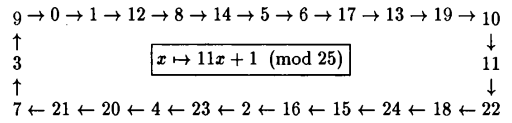
\includegraphics[width=0.8\linewidth]{image1}}
\end{figure}
... теперь должно быть более понятно, что обратимые по модулю $p^r$\linebreak
формы $a = 1 + kp$, суммы $S_{p^r}(а)$ и порядок $f$ тесно связаны между со­-\linebreak
бой. Однако, несмотря на все найденные соотнош ения, преобразование\linebreak
\newpage
$x \rightarrow 3x+1 \pmod{16}$ не является циклическим:
\begin{figure}[h]
\center{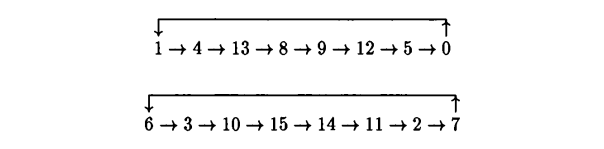
\includegraphics[width=1\linewidth]{image2}}
\end{figure}
\begin{predl}
\quad \;\;Пусть $p$ нечетное число, $k \ge 1$ и $r \ge 0$,.
\par  (\textit{i}) $x \equiv 1 \pmod{p^k} \Rightarrow S_{p^r}(x) \equiv p^r \pmod{p^{k+r}}.$
\par  (\textit{ii}) Если $x \equiv 1 + ap^k \pmod{p^{k+1}}$, то $x^{p^r} \equiv 1 + ap^{k+r}\pmod{p^{k+r+1}}$.\linebreak В частности,
$x \equiv 1 + ap \pmod{p^2}\rightarrow x^{p^r} \equiv 1 + ap^{r+1}\pmod{p^{r+2}$.}
\end{predl}
\begin{myproof}
\par (\textit{i}) Рассмотрим сначала случай $r = 1$. Тогда $x = 1 + vp^k$ для $v \in A$ и\linebreak
$$S_p(x)=1+(1+vp^k)+(1+vp^k)+...+(1+vp^k)^{p-1}$$
$$\equiv 1 + (1+vp^k) (1+2vp^k)+ ... + (1+(p-1)vp^k) \pmod{p^{k+1}}$$
$$\equiv p + vp^k(1 + 2 + ... + p - 1) \equiv p + vp^k\frac{p(p-1)}{2} \pmod{p^{k+1}}.$$
Откуда $S_p(x) \equiv p\pmod{p^{k+1}}$, так как $p$ нечетно. Для\linebreak
произвольного $r$ доказательство ведется по индукции, ибо\linebreak
$S_{p^{r+1}}(X) = S_{p^r}(X^p)S_p(X).$
\par  (\textit{ii})Имеем:
	$$x^{2^r} - 1 = (x - 1)S_{2^r}(x)=(a2^k + \alpha2^{k+1})(a2^k + \beta2^{k+r-1}=)$$
	$$=a2^{r+k}+\alpha \beta 2^{r+2k-1}+\alpha 2^{r+k+1}(1+\beta 2^{k-1})\equiv$$
	$$\equiv2^{k+r} \pmod{2^{r+k+1}}.\quad\quad\quad\quad\quad\quad\quad\quad\quad\;\;$$
\end{myproof}
\begin{mynotice}
Результаты, полученные в этом предложении, более\linebreak
тонкие, чем в предыдущем, но опираются на то, что $p$ нечетно.\linebreak
Следующие примеры показывают, что эти результаты неверны\linebreak
для четного $p$:
$$3\equiv 1\pmod{2}, \text{ но } S_2(3) \not\equiv 2 \pmod{4},$$
$$p = 2, x = 3, k = 1, r = 1;$$
$$(1 + 2)^2 \not\equiv 1 + 2^2\pmod{2^3}, p = 2, a = 1, k = 1, r = 1.$$
\end{mynotice}
\begin{beznomera}
\noindent \textbf{Применение}

Применим некоторые простые следствия предыдущего предложения\linebreak
к изучению структуры $U(\mathbb{Z}_{3^r})$. Итак, $р = 3$ и $а = - 1$. Тогда

Следовательно, $—2$ является элементом порядка $3^{r-1}$ по модулю $3^r$ . По­\linebreak
рядок $U(\mathbb{Z}_{3^r})$ равен $\phi (3^r) = 2 \times 3^{r-1}$, а значит, $—2$ не может быть\linebreak
элементом максимального порядка. Посмотрим, что дают предыдущие\linebreak
равенства для $2$ (хотя и без вычислений ясно, что $—1$ не является сте­-\linebreak
пенью $—2$):
$$(-2)^{3^{r-2}} = (1+ ap)^{3^{r-2}} \equiv 1 - 3^{r-1} \pmod{3^r}$$
$$\text{ и }$$
\noindent откуда, благодаря предложению 25, следует, что $2$ — образующий груп-\linebreak­
пы обратимых по модулю $3^r$ элементов.
\end{beznomera}
\begin{predl}
Пусть $r$ и $k$ — два целых числа, причем $k$ больше или равно 2.
\par (\textit{i}) Если $x \equiv 1 \pmod{2^k}$, то $S_{2^r}(x) \equiv 2^r \pmod{2^{k+r-1}}$. В частности,\linebreak
если $x \equiv 1 \pmod{4}$, то $S_{2^r}(x) \equiv 2^r \pmod{2^{r+1}}$.
\par (\textit{ii}) Если $x \equiv 1 + a2^k \pmod{2^{k+1}}$, то $x^{2^r} \equiv 1 + a2^{k+r+1}$.\linebreak
В частности, если $x \equiv 1 + 4a \pmod{8}$, то $x^{2^r} \equiv 1 + a2^{r+3}$.
\end{predl}
\begin{myproof}
\par (\textit{i}) Для $r = 1$ запишем $x = 1 + v2^k$, откуда $S_2(x) = 1 + (1+v2^k)$,\linebreak
что доказывает результат. Дальнейшее доказательство производится\linebreak
индукцией по $r$. Так как $S_{2^{r+1}}(x)= S_{2^{r}}(x^2)S_2(x)$=, то 
$$S_{2^{r+1}}(x)=(2^r+\alpha 2^{k+r-1}(2+\beta 2^{k})\equiv 2^{r+1},$$
ибо $r + 2k -1 \ge k + r$.
\par (\textit{ii})Имеем:
$$x^{2^r} - 1 = (x - 1)S_{2^r}(x) = (a2^{k} + \alpha 2^{k+1})(2^r+\beta 2^{k+r-1})=$$
$$= a2^{r+k}+\alpha \beta 2^{r +2k -1} + \alpha 2^{k+r+1}(1+\beta 2^{k-1})\equiv$$
$$\equiv a2^{k+r}\pmod{2^{k+r+1}},$$
ибо $r+2k-1\ge k + r +1$ (для $k \ge 2$).
\end{myproof}
\newpage
\noindent\textbf{Пример}

Пусть имеется рекуррентная последовательность
$$x_{n+1} = 13x_n + 1 \pmod{2^r}.$$
Применяя предыдущее предложение с $x = 13 \equiv 1 \pmod{4}$, находим, что\linebreak
$S_{2^{r-1}}(13) \equiv 2^{r - 1} \pmod{2^r}$, в то время как $S_{2^r}(13) =\equiv 0 \pmod{2^r}$. Это\linebreak
означает, что аффинное отображение $x \rightarrow 13x+1 \text{ mod } 2^r$ в точности\linebreak
порядка $2^r$. Это хорошо видно на следующем примере:
\begin{figure}[h]
\center{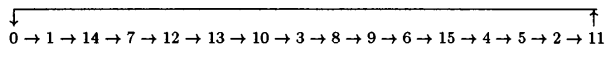
\includegraphics[width=1\linewidth]{image5}}
\end{figure}

Вопрос в том,всегда ли верно, что отображение порядка $2^r$ на $2^r$\linebreak
элементах является циклом длины $2^r$ ? Отображение $(1) (23) (456)$ пере­-\linebreak
ставляет $6$ элементов, имеет порядок $6$, но не является циклом!
\paragraph{3.4.2 Группа обратимых элементов $\mathbb{Z}/2^r\mathbb{Z}$}
\begin{thm}
\par\quad\;\;(\textit{i}) Группа $U(\mathbb{Z}_{2^r}$имеет порядок $2^{r-1}$. Группа $U(\mathbb{Z}_2)$ тривиальна,\linebreak
группа $U(\mathbb{Z}_4)$ — циклическая порядка $2$ и порождена элементом $3 = — 1$.
\par  (\textit{ii}) Предположим, что $r\ge2$. Пусть $\pi$ — отображение $U(\mathbb{Z}_{2^r})$  в\linebreak
$U(\mathbb{Z}_{4})$, определенное по правилу $\pi(x) = x\pmod{4}$. Тогда ограничение $\pi$ на\linebreak
$\{ — 1,1\}$ — изоморфизм на $U(\mathbb{Z}_4)$ и имеется разложение\linebreak
$U() = \text{Ker }\pi  х {—1, 1}$, которое задается следующим образом:
$$x = x \times 1, \text{ если } x \equiv 1 \pmod{4},$$
$$x = (-x) \times (-1), \text{ если } x \equiv 3 \pmod{4}$$
Кроме того, $\ker\pi$ - циклическая группа порядка $2^{r-2}$.
\par  (\textit{iii}) Предположим,что $r > 2$. Пусть $x = 1\pmod{4}$. Тогда\linebreak
$x\pmod{2^r}$ является порождающим $\text{Ker }\pi$ тогда и только тогда, когда\linebreak
$x\not\equiv 1 \pmod{8}$. Например, $5$ — образующий $\text{Ker }\pi$ по модулю $2^r$ для\linebreak
всякого $r\ge2$ (как мы это видели в разделе 1).
\par  Итак, при $r > 2$ группа $U(\mathbb{Z}_{2^r})$ порядка $2^{r-1}$ является прямым произ­-\linebreak
ведением циклической группы порядка $2^{r-2}$, порожденной элементом $5$,\linebreak
и циклической группы порядка $2$, порожденной элементом $—1$.
\end{thm}
\pagebreak
\begin{myproof}
\par  (\textit{ii}) То, что $\Ker{\pi}$ циклическая, следует из пункта (\textit{iii}) при $r > 2$\linebreak
и из того, что $\pi$ --- изоморфизм при $r = 2$.
\par  (\textit{iii}) Пусть $x$ — такое целое число, что $x \equiv 1 (\text{mod } 4)$. Обозна­-\linebreak
чим через $\overline{x}$ его класс по модулю $2^r$ и запишем $x = 1 + 4a$ с
$a \in \mathbb{Z}$. Так как $x$ принадлежит группе $\Ker{\pi}$, порядок которой равен\linebreak
$2^{r-2}$, то $x^{2^{r-2}} \equiv 1 (\text{mod } 2^r)$. Кроме того, согласно предложению 32,\linebreak
$x^{2^{r-3}} \equiv 1 + a2^{r-1} (\text{mod } 2^r)$ и, следовательно, $x^{2^{r-3}} \not\equiv 1 (\text{mod } 2^r)$ то­-\linebreak
гда и только тогда, когда $a \not\equiv 0 (\text{mod } 2)$. Это означает, что порядок\linebreak
$x$ равен $2^{r-2}$ тогда и только тогда, когда $x \not\equiv 1 (\text{mod }8)$.
\end{myproof}
\paragraph{3.4.3 Группа обратимых элементов	$\mathbb{Z}/p^r\mathbb{Z}$ при нечетном $p$}
%\newtop{Группа обратимых элементов	$\mathbb{Z}/p^r\mathbb{Z}$ при нечетном $p$}
\begin{lemma}
Предложение 30 (\textit{ii}) позволяет определить отображение $\chi_{r,k}$ из\linebreak
$U(\mathbb{Z}_{p^r})$ в $U(\mathbb{Z}_{p^{r+k}})$ по правилу $\chi_r,k(x mod р^{r+k}) = x^{p^k}\text{mod }р^{r + k}$. Позво-­\linebreak
ляя себе небольшую вольность, будем это иногда обозначать через\linebreak
$\chi_{r,k}(x)=x^{p^k}$.
\end{lemma}
\begin{predl}
Пусть $\pi$ — естественный гомоморфизм $U(\mathbb{Z}_{p^r})$ на $U(\mathbb{Z}_p)$. Обозначим\linebreak
через $\chi = \chi_{1,r-1}$ отображение из $U(\mathbb{Z}_p)$ в $(U(\mathbb{Z}_{p^r})$.
 
\par  (\textit{i}) Отображение $\chi$ есть сечения $\pi: \pi \textopenbullet \chi = Id$. В частности, $\chi$ инъ-\linebreak
ективно, а $\pi$ сюрьективно.
\par  (\textit{ii}) Благодаря разложению $x = {(x^{p^{r-1}})^{-1}} \times x^{p^{r-1}}$, имеем $U(\mathbb{Z_{p^r}})=$$\ker\pi \times \im \chi.$
\par  (\textit{iii}) Кроме того $\ker \pi$ --- группа порядка $p^{r-1}$, состоящая из таких\linebreak
элементов $x \in U(\mathbb{Z}_{p^r})$, что $x \equiv 1 (\mod p)$, a $\im x$ — группа порядка\linebreak
$p — 1$, образованная $q$-ми степенями элементов из $U(\mathbb{Z}_{p^r})$, где $q = p^r - 1$\linebreak
($\im x$ изоморфна $U(\mathbb{Z}_p)$).
\end{predl}
\begin{myproof}
 
\par  (\textit{i}) Пусть $x \in \mathbb{Z} - p\mathbb{Z}$, т.е. $x$ обратимо по модулю $p^k$ для любого $k$.\linebreak
Тогда
$$\pi \textopenbullet \chi(x\mod p) = \pi (x^{p^{r-1}}\mod p^r)=^{p^{r-1}}\mod p=x\mod p,$$
$$\text{так как } y^p \equiv y (\mod p).$$
\newpage
\par  (\textit{ii}) Отображение $r = 
\chi \textopenbullet \pi$ является проекцией $U(\mathbb{Z}_{p^r})$, т.е. $r \textopenbullet r = r$.\linebreak
Следовательно, имеем классическое разложение в прямое произве-\linebreak­
дение ядра и образа:
$$U(\mathbb{Z}_{p^r})=\text{Ker }r \times \im r, \text{ по правилу: }x = (xr(x)^{-1})\times r(x)$$
То, что разложение $\text{Ker }r \times \im r$имеет место и что оно единственно,\linebreak
сразу следует из свойства $r \textopenbullet r = r$. В нашем случае $\chi$ инъективно,\linebreak
а значит, $\text{Ker }r = \text{Ker } \pi$, а так как $\pi$ сюръективно, то $\im r= \im \chi$.\linebreak
Вычисляя $x * r (x)^{-1}$ и $r(x)$, получим выражения, записанные в усло­-\linebreak
вии.
\par  (\textit{iii}) $\text{Ker }\pi$ состоит из элементов $U(\mathbb{Z}_{p^r})$ таких, что $x \equiv 1 (\mod р)$, и\linebreak
нетрудно сосчитать количество таких элементов: $p^{r - 1}$ . Таким обра-\linebreak
зом, снова получили функцию Эйлера для $p^r$.
\end{myproof}
\begin{predl}
Пусть $p$ --- нечетное простое число, а $r > 0$.
 
\par  (\textit{i}) Элемент $1 - p$ имеет порядок $p^{r-1}$ в $\text{Ker }\pi$. Другими словами, $1-p$\linebreak
порождает $\text{Ker }\pi$.
\par  (\textit{ii})Гомоморфизм $\chi_{r,k}$ группы $U(\mathbb{Z}_{p^r})$ инъективен.
\end{predl}
\begin{myproof}
 
\par  (\textit{i}) Порядок $\text{Ker }\pi$ равен $p^{r-1}$ и, очевидно, $1 — p$ принадлежит $\text{Ker }\pi$.\linebreak
Следовательно, порядок $1 — p$ делит $p^{r - 1}$. Кроме того, используя\linebreak
предложение 31 (i), имеем:
$$(1-p)^{p^{r-2}}\equiv 1 - p^{r-1} \not\equiv 1 (\mod p^r).$$
Значит, $1 - p$ имеет порядок $p^{r-1}$.
\par  (\textit{ii}) Достаточно доказать, что инъективен $\chi_{r,1}$. Действительно,\linebreak
$$\chi_{r,k} = \chi_{r+k-1,1}\textopenbullet...\textopenbullet\chi_{r+1,1}\textopenbullet\chi_{r,1}.$$
Для этого же достаточно показать, что из $x^p \equiv 1 (\mod p^{r+1})$ сле­-\linebreak
дует $x \equiv 1 (\mod p^r)$. Пусть $x$ таково, что $x^p \equiv 1(\mod p^{r + 1})$. Тогда\linebreak
$x^p \equiv 1 (\mod p)$, а значит, $x \equiv 1 (\mod p)$. Согласно предложению 31\linebreak
(i) имеем $S_p(x) = p (\mod p^2 )$ и тем более $S_p (x) \not\equiv 0 (\mod p^2 )$. Из\linebreak
равенства $x^p -1 = (x - 1)S_p(x)$ и того, что по условию левая часть\linebreak
равенства делится на $p^{r + 1}$ , a $S_p(x)$ не делится на $p^2$ по только что
доказанному, заключаем, что $r —1$ делится на $p^r$. Что и требовалось
доказать.
\end{myproof}
\begin{mynotice}
Элемент $1 + kp$ также порождает $\text{Ker }\pi$, если $k \not\equiv 0$\linebreak $(\mod p)$.

Отображение $\mathbb{Z}$ в $U(
\mathbb{Z}_{p^2})$, которое каждому числу $b$ ставит в\linebreak
соответствие $1 — bp$, является гомоморфизмом, чье ядро — $p\mathbb{Z}$, а\linebreak
образ — $\text{Ker }\pi$. Это отображение индуцирует изоморфизм $\mathbb{Z}_p$ и\linebreak
$\text{Ker }\pi$. Если $x \in \mathbb{Z} — p\mathbb{Z}$, то разложение $U(\mathbb{Z}_{p^2})$, введенное в предло­-\linebreak
жении 35, позволяет записать $x = x^p(x^{p-1})^{-1}$. По малой теореме\linebreak
Ферма 
$x^{p-1}=1+a_xp$, а значит $x \equiv x^p(1-a_xp) (\mod p^2)$, откуда\linebreak
$$x \equiv x^p(1-p)^{a_x}(\mod p^2).$$
Это позволяет заключить, что в $U(\mathbb{Z}_{p^2})$ компонента $x$, принадле-\linebreak­
жащая $\text{Ker }\pi$, есть степень $a_x$ образующей $1 — p$ ядра $\text{Ker }\pi$.
\end{mynotice}

Предыдущее предложение позволяет полностью определить струк­-\linebreak­
туру $U(\mathbb{Z}_{p^к})$ для нечетного простого $P$. Так как $p — 1$ и $p^r - 1$ взаимно\linebreak­
просты и группа $U(\mathbb{Z}_{p^r})$ — прямое произведение циклических групп\linebreak­
порядков $p — 1$ и $p^r - 1$, то она изоморфна $\mathbb{Z}_{p^{r-1}(p-1)}$ и циклична.
\begin{thm}
Пусть $p$ — нечетное простое число, а $r$ - строго положительное целое число.
 
\par  (\textit{i}) Элемент $1 - p$ имеет порядок $p^{r-1}$ в $U(\mathbb{Z}/{p^r}\mathbb{Z})$.
\par  (\textit{ii}) Группа $U(\mathbb{Z}/{p^r}\mathbb{Z})$ изоморфна прямому произведению подгруппы
порядка $p^{r-1}$, порожденной элементом $1-p$, и подгруппы порядка $p — 1$,
образованной $q$-ми степенями элементов $U(\mathbb{Z}/{p^r}\mathbb{Z})$, где $q = p^{r-1}$ . Вторая
подгруппа изоморфна $U(\mathbb{Z}/{p^r}\mathbb{Z})$.
\par  (\textit{iii}) Группа $U(\mathbb{Z}/{p^r}\mathbb{Z})$ --- \textbf{циклическая} порядка $p^{r-1}(p-1)$.
\end{thm}


\noindent\textbf{Пример}
\\

В таблице 4 дана группа обратимых по модулю 125 элементов, разло­-\linebreak­
женная согласно предыдущему изложению. В первом столбце находится\linebreak­
образ $\chi$ , а в первой строке --- ядро $\pi$.

Первый столбец состоит из 25-х степеней чисел по модулю 125 и\linebreak­
изоморфен$U(\mathbb{Z}_5)$. При этом \textit{изоморфизме} элементы 57 и 68 соответ­-\linebreak­
ствуют образующим группы $%U(\mathbb{Z}_5)$. Кроме того, теперь легко опреде­-\linebreak­
лить образ любого элемента из $%U(\mathbb{Z}_125)$ под действием $\chi$:это элемент\linebreak­
первого столбца, который имеет тот же остаток по модулю 5.
\newpage
\end{document} 